\subsection{Authorization Levels}
\begin{enumerate}
\item Admin \\
Users that are configured with an Authorization Level of Admin will have the ability to access, add, and re-configure:
\begin{itemize}
\item Users
\item Hosts
\item Services
\item Components
\item Configuration Wizards
\item Dashlets
\item Program Settings
\item Security Credentials
\end{itemize}
\item User
\\
Users with an Authorization Level of User will only be able to see and modify hosts and services for which they are a notification contact.
\end{enumerate}
\subsection{User Security Settings}
Administrators may grant users additional rights beyond the default permissions they have in Nagios XI.
\begin{itemize}
\item Can see all hosts and services \\
The user can see all hosts and services that are being monitored.
\item Can (re)configure hosts and services \\
The user can re-configure and delete existing hosts and services(which they can see) from the monitoring configuration, and add new hosts and services to the monitoring configuration.
\item Can control all hosts and services \\
The user can see and submit commands(e.g. disable notifications) for hosts and services.
\item Can see/control monitoring engine \\
The user can see and control(e.g.shutdown or restart) the monitoring engine.
\item Can access advanced features \\
The user can see the Advanced tab when viewing the details of hosts and services, can see some menu items and options that are not usually suitable for basic users. 
\item Has read-only access \\
It removes the user's ability to submit commands(e.g. diable notifications) for hosts and services. It also prevents them from re-configuring existing or adding new hosts and services.
\end{itemize}
\begin{figure}[htp]
\centering
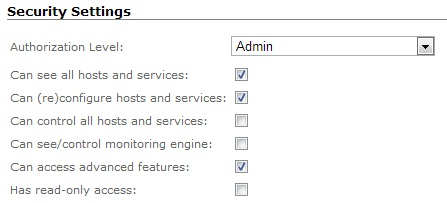
\includegraphics[width=0.6\textwidth]{Christof/Bilder/Security}
\caption{Security Settings}
\label{fig:SecuritySettings}
\end{figure}